%!TEX root=rapport.tex

\section{Interprétation des résultats obtenus}

\subsection{Résultats finaux}

Pour étudier les résultats que notre programme nous retourne, nous avons utilisé
un \textit{dotmatcher}.
Le principe du dotmatcher est de comparer deux séquences $s$ et $t$ données en
entrée: le dotmatcher parcourt les séquences en comparant chaque nucléotide
entre eux.  Lorsqu'un correspondance est faite, un point est tracé sur un
graphique. Une option, appelée \textit{thresold} peut être ajustée pour dissiper
le bruit.

\FloatBarrier

%\begin{center}
	%\begin{figure}
		%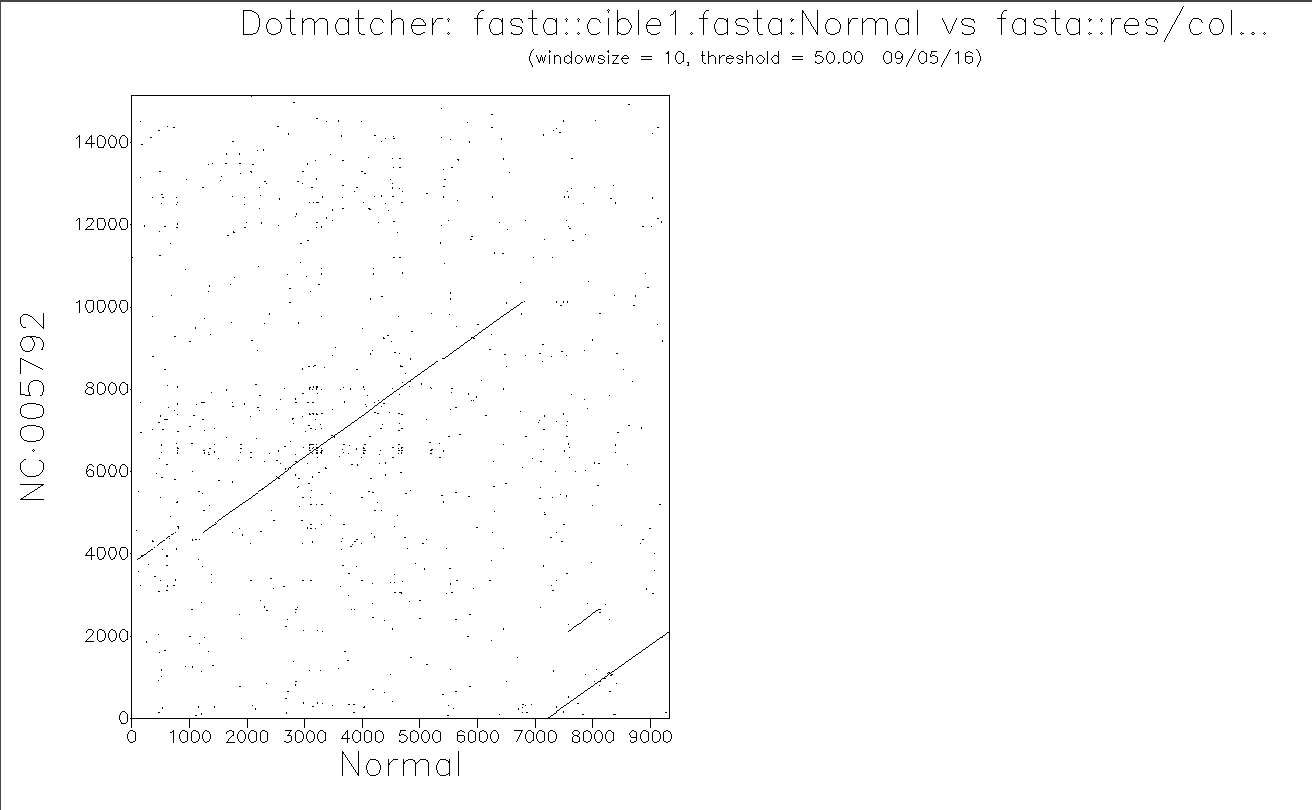
\includegraphics[scale= 0.4]{../res/cible1.png}
		%Exemple de graphique obtenu à partir du dotmatcher
	%\end{figure}
%\end{center}


Pour chaque nucléotide $s_{i}$ de la séquence $s$ et chaque nucléotide $t_{j}$
de la séquence $t$, le dotmatcher va tracer un point s'il y a une correspondance
entre les deux nucléotides.

Pour chaque comparaisons de séquences, nous obtenons donc un rectangle de
points. Sur l'axe X, nous avons la longueur de la séquence que nous devons
obtenir, et sur l'axe Y, nous avons la longueur de la séquence que nous avons
obtenue.

Nous souhaitons, à travers ces graphiques, étudier le comportement de notre
séquence obtenue en regardant si chaque morceau de la séquence cible est bien
atteinte, ceci se remarquant à travers les morceaux de droites. Pour cela, il
suffit de projeter chaque droite obtenue sur l'axe X et regarder si l'ensemble
recouvre globalement la séquence de départ.

\subsubsection*{Cible 1}

Au niveau de la première cible, nous remarquons d'abord que la séquence que nous
avons obtenue est trop longue ($\simeq$ 14 000 vs $\simeq$ 9000).

Les résultats sont meilleurs pour le premier que pour son complémentaire
inversé. Le recouvrement du premier est presque global, les intervalles non
couverts se trouvant aux alentours de 1000 et 7000.

Nous remarquons, à travers les droites, que nous avons de longues successions de
correspondances.

\begin{figure}[!ht]
	\begin{minipage}[r]{.46\linewidth}
		\begin{center}
		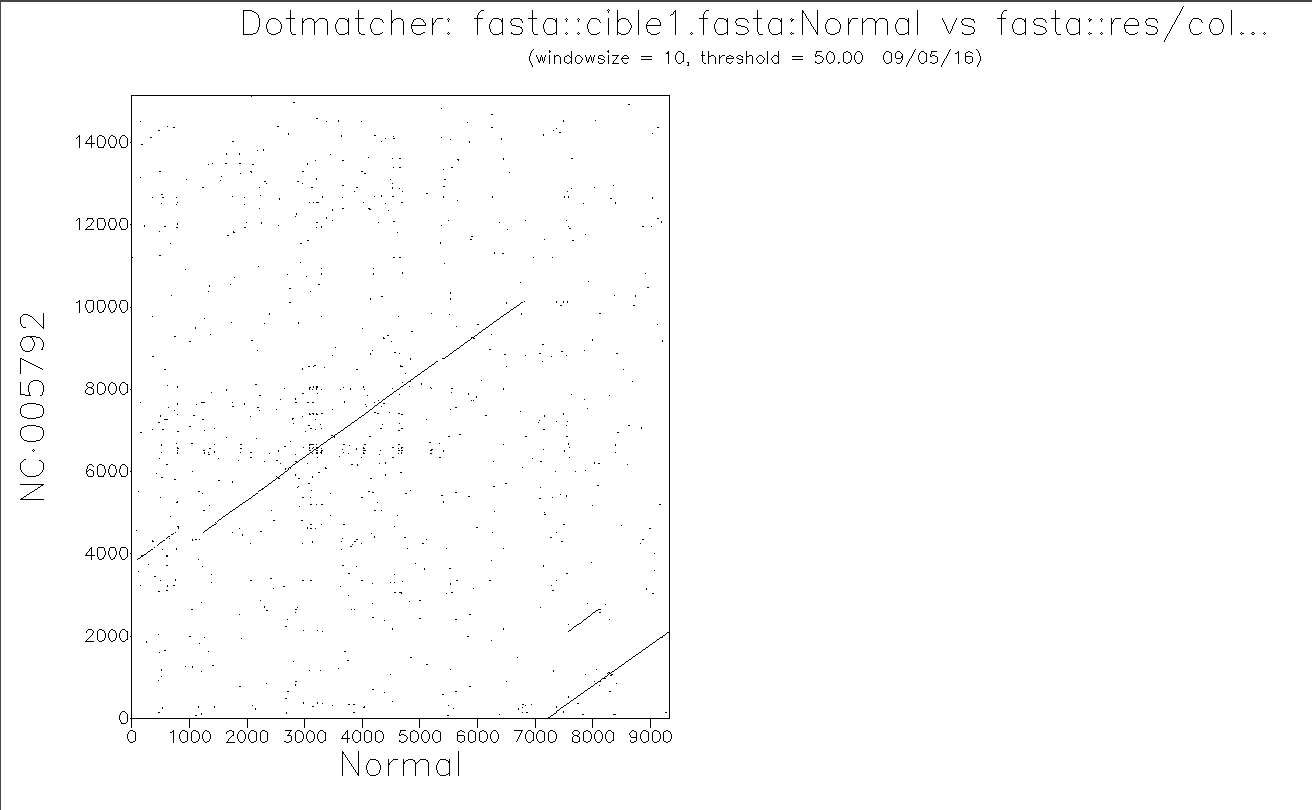
\includegraphics[scale= 0.4]{../res/cible1.png}
		Résultat de la collection 1
	\end{center}
\end{minipage} \hfill
\begin{minipage}[c]{.46 \linewidth}
	\begin{center}
			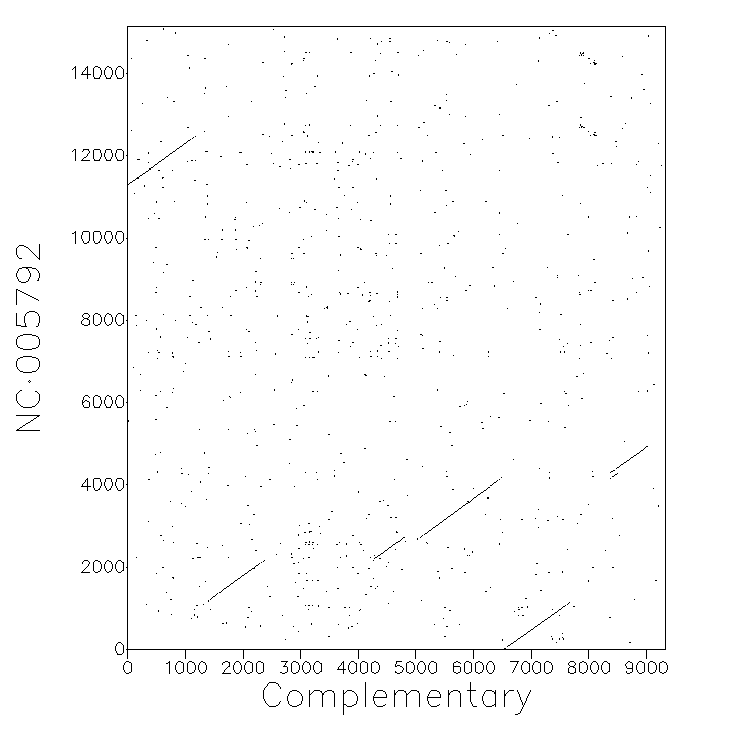
\includegraphics[scale= 0.4]{../res/cible1-ic.png}
			Résultat de la collection 1, complémenté et inversé
		\end{center}
	\end{minipage}
	\caption{Résultat de la collection 1}
\end{figure}

\FloatBarrier

\subsubsection*{Cible 2}

Quant à la seconde cible, bien que nous obtenons des résultats assez éparpillés,
le recouvrement est assez grand, aussi bien pour le normal que son
complémentaire inversé.
Le graphique du complémentaire inversé comprend tout de même plus de droites, et
plus longues aussi que le normal.

Nous obtenons également une trop grande séquence: la cible est contient environ
118000 nucléotides tandis que notre alignement en contient 190000.

\begin{figure}[!ht]
	\begin{minipage}[r]{.46\linewidth}
		\begin{center}
		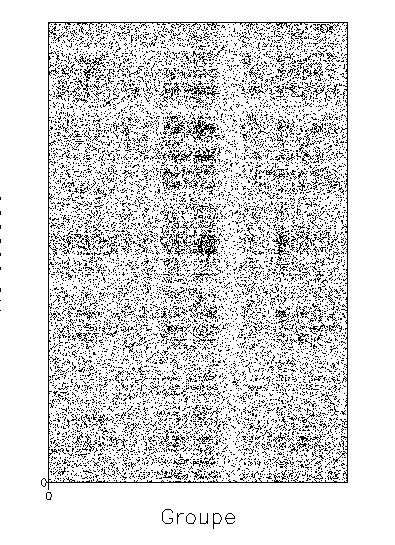
\includegraphics[scale=0.25]{../res/cible2.png}
		Résultat de la collection 2
	\end{center}
\end{minipage} \hfill
\begin{minipage}[c]{.46 \linewidth}
	\begin{center}
			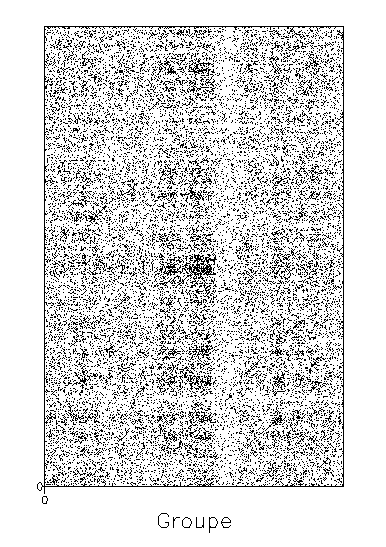
\includegraphics[scale=0.25]{../res/cible2-ic.png}
			Résultat de la collection 2, complémenté et inversé
		\end{center}
	\end{minipage}
	\caption{Résultat de la collection 2}
\end{figure}

\FloatBarrier

\subsubsection*{Cible 4}

Les résultats pour la cible 4 sont plutôt satisfaisantes comme pour les cibles 1
et 5. Nous obtenons un recouvrement quasi-global ainsi qu'une longue droite
recouvrant environ 65\% de la séquence cible.

Pour son complémentaire inversée, le recouvrement est plus éparpillé mais reste
tout de même assez global.

Comme les 2 premières séquences, nous obtenons une séquence trop longue.

\begin{figure}[!ht]
	\begin{minipage}[r]{.46\linewidth}
		\begin{center}
		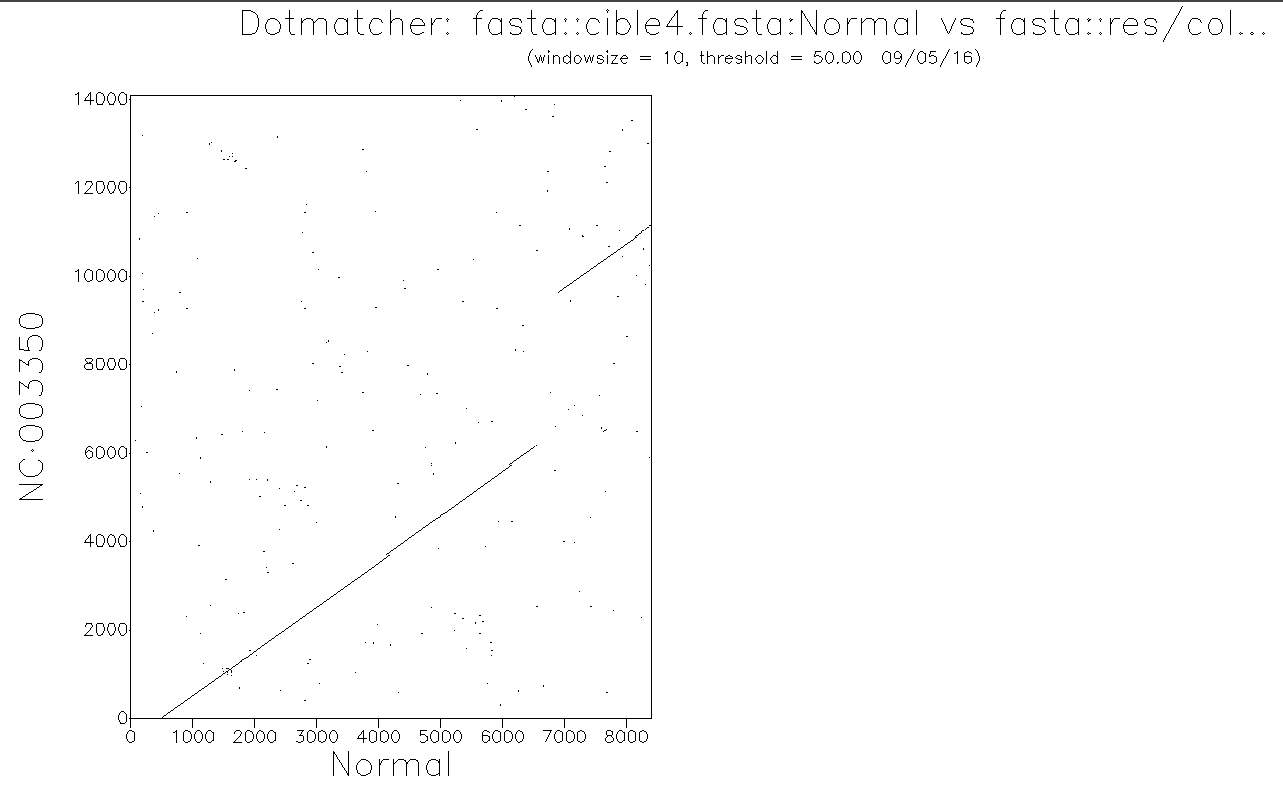
\includegraphics[scale= 0.4]{../res/cible4.png}
		Résultat de la collection 4
	\end{center}
\end{minipage} \hfill
\begin{minipage}[c]{.46 \linewidth}
	\begin{center}
			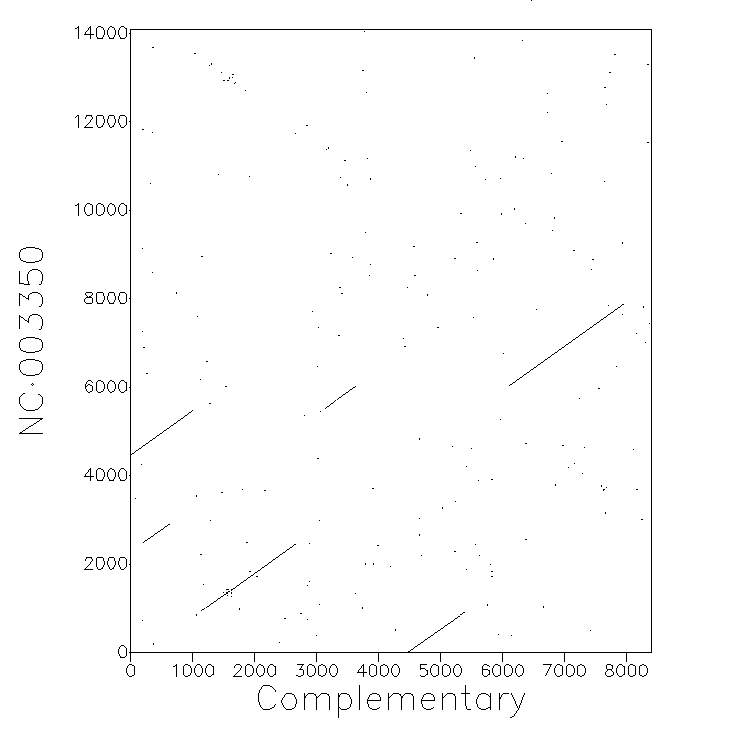
\includegraphics[scale= 0.4]{../res/cible4-ic.png}
			Résultat de la collection 4, complémenté et inversé
		\end{center}
	\end{minipage}
	\caption{Résultat de la collection 4}
\end{figure}

\FloatBarrier

\subsubsection*{Cible 5}

Pour la dernière cible, la 5, nous obtenons aussi plusieurs segments de droites,
plus ou moins grands, recouvrant la majorité de la séquence cible (un peu plus
de 90\%). Les endroits où les deux séquences ne matchent pas se situent aux
alentours de 3000 et 7500. Le complémentaire inversé remplit également une bonne
partie de la séquence cible mais il y a plus d'intervalles où les séquences ne
se correspondent pas.

Comme pour les séquences précédentes, notre algorithme nous renvoie une séquence
trop longue (environ 6000 nucléotides de trop).

\begin{figure}[!ht]
	\begin{minipage}[r]{.46\linewidth}
		\begin{center}
		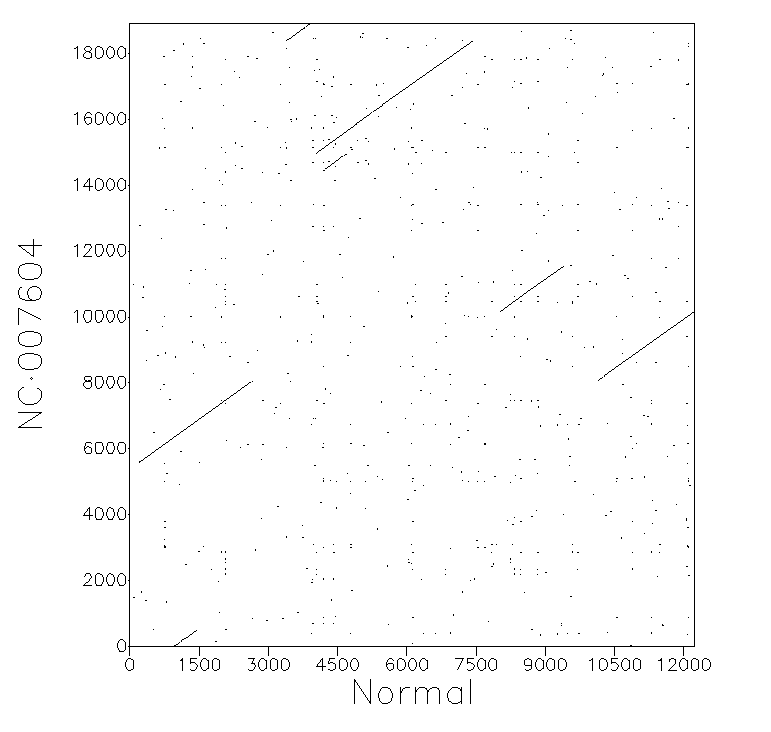
\includegraphics[scale= 0.4]{../res/cible5.png}
		Résultat de la collection 5
	\end{center}
\end{minipage} \hfill
\begin{minipage}[c]{.46 \linewidth}
	\begin{center}
			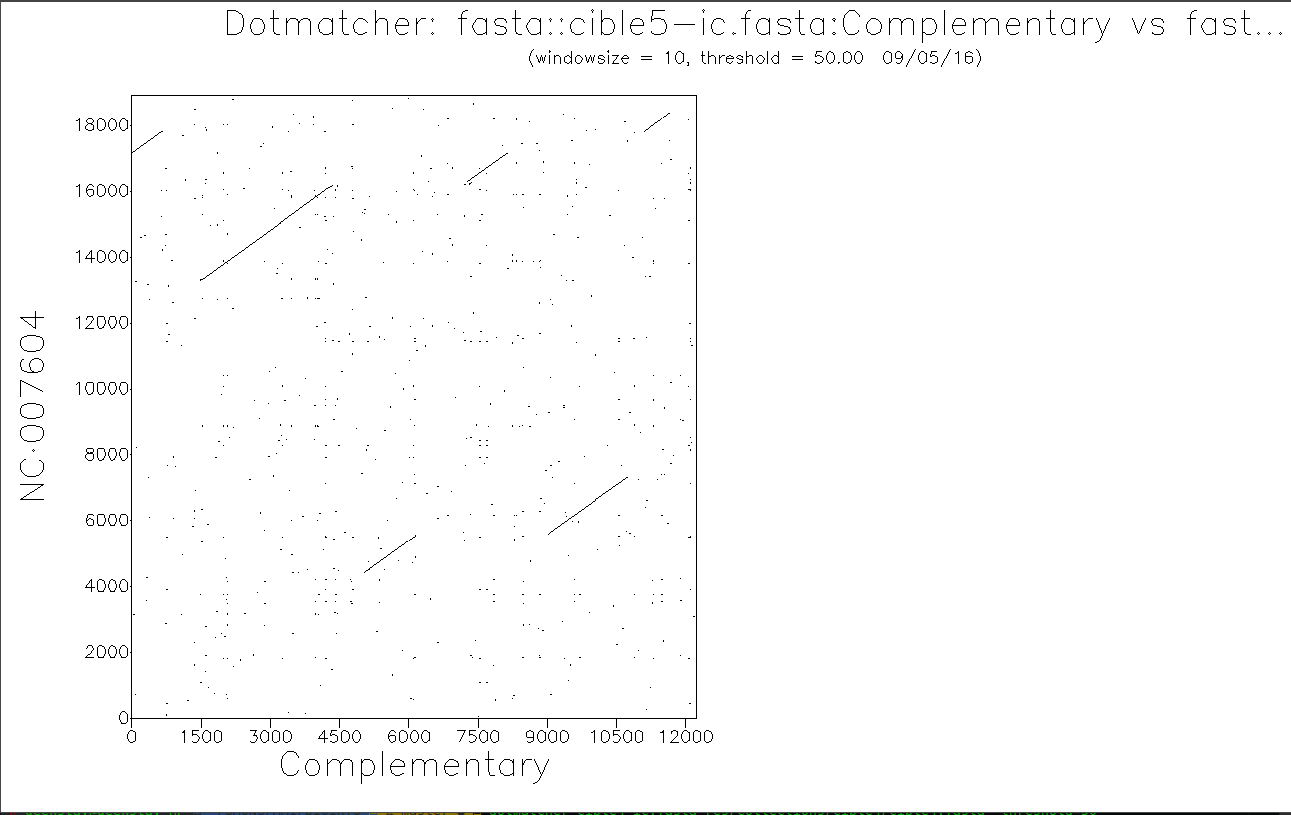
\includegraphics[scale= 0.4]{../res/cible5-ic.png}
			Résultat de la collection 5, complémenté et inversé
		\end{center}
	\end{minipage}
	\caption{Résultat de la collection 5}
\end{figure}

\FloatBarrier


\subsubsection*{Interprétation Générale}


\subsection{Autres implémentations}

Nous avons également tenté de changer l'implémentation du Greedy en changeant
le comparateur d'arcs, en prévilégiant les nombres de gaps finaux et initiaux
dans l'alignement semi-global ainsi qu'en propageant les gaps à la fin. Ces
méthodes ont donné des résultats différents mais pas aussi bons que ceux obtenus
initialement.

Par exemple, lorsque deux arcs ont un même score, nous avons tenté de
privilégier les arcs qui ont une plus longue sous-séquence commune Cette méthode
ne nous a pas donné de mauvais résultats mais ils étaient moins bons.

Dans le code soumis, nous avons prévilégié, lors de l'alignement semi-global,
l'alignement avec le moins de gaps finaux et initiaux, c'est-à-dire en
prenant le dernier maximum pour la dernière colonne et la dernière ligne. Nous
avons tenté de prendre le premier maximum pour chacun d'entre eux, mais cela n'a
pas donné de meilleurs résultats.

%Explication de la propagations des gaps à la fin.
